\section{Introduction}
La industria agroalimentaria está formada por cadenas de suministro complejas: sistemas interconectados de organizaciones, personas, actividades, datos y cadenas de suministro \cite{traza1}.
Este ecosistema puede presentar beneficios económicos, sociales y ambientales pero también grandes riesgos \cite{traza2}.
La seguridad alimentaria, la responsabilidad social,
junto con el avance de las tecnologías habilitadoras digitales, que impulsan la cuarta revolución industrial, ofrecen tendencias y recursos tecnológicos que favorece la integración de soluciones beneficiosas tanto para el mercado como para los consumidores. A pesar de estos avances y beneficios, a menudo hay preocupaciones sobre la implementación tecnológica. Para que las cadenas de suministro de alimentos sean verdaderamente rastreables, y para que los beneficios sean sentidos por todos dentro de la cadena de valor de los alimentos, el uso de las tecnologías propuestas debe ser universal. Existen barreras como el precio, la accesibilidad y la aceptación. Soluciones como la adopción de paradigmas prometedores como el blockchain (sistema descentralizado para registrar y proteger transacciones y datos) está limitada debido a la falta de "madurez tecnológica" \cite{blockchain1}. Otros factores podrían incluir la falta de confianza de las pequeñas empresas o granjas de los países en desarrollo, que consideran que la digitalización de los procesos es "costosa y complicada" \cite{agro1}.
En este trabajo se realizará el análisis de las tecnologías de comunicación más adecuadas para desarrollar servicios de trazabilidad digital en la cadena de valor agroalimentaria (sección2). A continuación se propone el diseño de un sistema de trazabilidad que integre a los diferentes actores detectados en la cadena de valor y las tecnologías necesarias para desplegar los servicios definidos con el objetivo de mejorar los inconvenientes indicados y evitar las barreras detectadas (sección3). Una vez realizado el diseño se implementa de forma experimenta un prototipo funcional (sección4). Finalmente se evalúan los resultados y se enumeran las conclusiones del trabajo (sección 5).

\begin{figure}[tp]
\centering
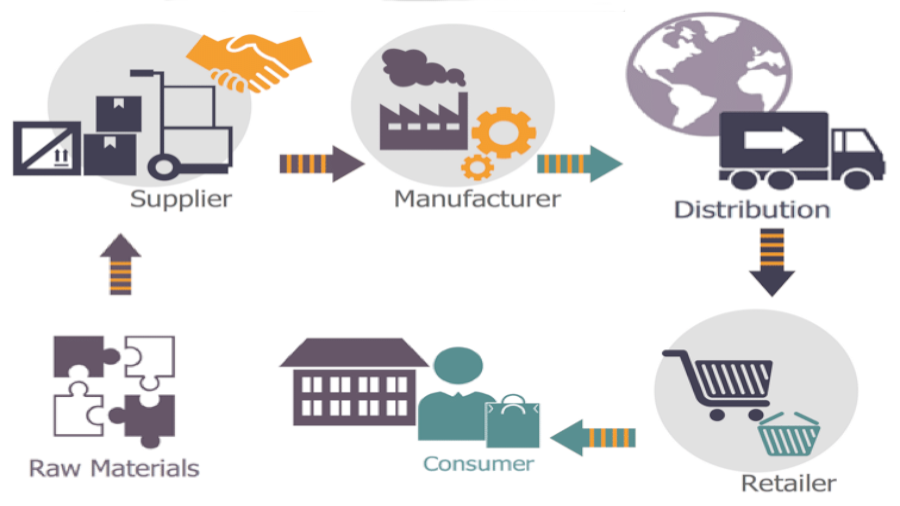
\includegraphics[width=8cm]{figures/Traza1.png}

\caption{Escenario de trazabilidad}
\label{escenario}
\end{figure}

\section{Related Work}

Las tecnologías de digitalización para el escenario planteado abarcan la cadena de valor indicada en la Figura \ref{escenario}.

\section{System Design}
La aceptación de la tecnología, el precio de la implantación, la accesibilidad a las soluciones tecnológicas, la dificultad en el uso o su propio mantenimiento son factores que están retrasando el despliegue y aprovechamiento de los beneficios de la digitalización en la trazabilidad. Del análisis de estos factores y del estudio del estado de la tecnología se propone un modelo que reduzca las barreras mediante la integración, adaptación y despliegue coordinado de diferentes tecnologías. 

\subsection{The First Layer}
\Blindtext

\subsection{The Second Layer}
\Blindtext

\section{Evaluation}
\Blindtext

\section{Conclusion}
\blindtext

